\documentclass{article}
\usepackage{haldefs}
\usepackage{notes}
\usepackage{lwdefs}
\usepackage{graphicx}
\usepackage{url}
\usepackage{textcomp}
\usepackage{enumitem}
\usepackage{subfig}
\usepackage{hyperref}
%\usepackage{/home/sci/weiliu/packages/breakurl/breakurl}

\usepackage{amsmath}
\usepackage{verbatim}
\usepackage{natbib}
\usepackage{algorithmic}
\usepackage{algorithm}
\usepackage{color}
\usepackage{mdwlist}
\usepackage{tikz}
\usetikzlibrary{positioning}
\usetikzlibrary{arrows,fit,decorations.pathmorphing,backgrounds,positioning,shapes.misc,calc,trees,positioning,chains,shapes.geometric,decorations.pathreplacing,decorations.pathmorphing,shapes,matrix,shapes.symbols,shadings,shadows}

\hypersetup{
  % bookmarks=true,         % show bookmarks bar?
    unicode=false,          % non-Latin characters in Acrobat’s bookmarks
    pdftoolbar=true,        % show Acrobat’s toolbar?
    pdfmenubar=true,        % show Acrobat’s menu?
    pdffitwindow=false,     % window fit to page when opened
    pdfstartview={FitH},    % fits the width of the page to the window
    pdftitle={Monte Carlo Expectation Maximization},
    pdfauthor={Wei Liu},     % author
    pdfsubject={Monte Carlo Expectation Maximization},   % subject of the document
    pdfcreator={Wei Liu},   % creator of the document
    pdfproducer={Producer}, % producer of the document
    pdfkeywords={Monte Carlo, Expectation Maximization}, % list of keywords
    pdfnewwindow=true,      % links in new window
    colorlinks= true,       % false: boxed links; true: colored links
    linkcolor=red,          % color of internal links
    citecolor=green,        % color of links to bibliography
    filecolor=magenta,      % color of file links
    urlcolor=cyan           % color of external links
}


\setlength{\oddsidemargin}{0 in}
\setlength{\evensidemargin}{0 in}
\setlength{\topmargin}{-0.6 in}
\setlength{\textwidth}{6.5 in}
\setlength{\textheight}{9 in}
\setlength{\headsep}{0.5 in}
\setlength{\parindent}{0 in}
\setlength{\parskip}{0.1 in}



\begin{document}
\title{Monte Carlo Expectation Maximization}
\author{Wei Liu}
\maketitle
\tableofcontents

\section{Prior Distribution}

The Gibbs distribution is defined as
\begin{align}
  P(\vec f) = \frac{1}{Z} \exp\{-U(\vec f)\},
\end{align}
where the energy function $U$ is given as
\begin{align}
  U(\vec f) = \sum_{i \in \mathcal{S}} V_1 (f_i) + \sum_{(i,j) \in \mathcal{E}} V_2 (f_i, f_j)
\end{align}
$V_1$ is one site clique potential, and is defined as $V_1(f_i) = \alpha(
f_i)$. $V_2$ is the two site clique potential. For multiple labels
$\mathcal{L} = \{1,\dots, K\}$, we can use \emph{Potts model} defined
as
\begin{align}
  V_2 (f_i, f_j) &= w_{ij} T(f_i \neq f_j)
\end{align}
where $T$ is $1$ if its argument is true, and $0$
otherwise\citep{boykov2002fast}. $w_{ij}$ can be different for each
pair of neighboring pixels. For simplicity we assume it is constant
for all neighboring pixels, and let $w_{ij} = \beta$. $\alpha$ is used
to give the preference to some labels. For now we just set it to
zero. The Gibbs distribution is given as
\begin{align}
  U(\vec f) &= \beta \sum_{(i,j) \in \mathcal{E}}T(f_i \neq f_j) \\
  P(\vec f) &= \frac{1}{Z} \exp \{  - \beta \sum_{(i,j) \in \mathcal{E}}T(f_i \neq f_j)\}.
\end{align}
For a single pixel $f_i$ (because of the Markov-Gibbs equivalence),
\begin{align*}
  U(f_i) &= \beta \sum_{j \in \mathcal{N}_i} T(f_i \neq f_j)  = \beta S_i^n\\
  P(f_i | f_{-i} ) &= P(f_i | f_{\mathcal{N}_i}) \\
  &= \frac{\exp\{- \beta \sum_{j\in \cN_i}T(f_i \neq f_j)\}}{\sum_{f_i \in \cL}\exp\{ - \beta \sum_{j\in \cN_i}T(f_i \neq f_j)\}} \\
&=   \frac{\exp \{ -\beta S_i^n(f_i)\}}{\sum_{f_i \in \mathcal{L}} \exp \{ -\beta S_i^n(f_i) \}}
\end{align*}

$f_{-i}$ is the labeling for all data points except $i$. $\beta > 0$ means adjacent pixels should have same labeling. For convenience we define $S_i^n (f_i) = \sum_{j\in \mathcal{N}_i} T(f_i \neq f_j) $.

\section{Sampling From Prior Distribution}

To generate synthetic image we need to sample from MRF to get a label image.  We can use Metropolis Sampler to generate a sample image from prior distribution $P(\vec f)$ as follows:
\begin{itemize}
  \item[1.] Start with initial label image $\vec f^1$.
  \item[2.] Given previous sample $\vec f^{n}$, generate a new sample $\vec w$ by drawing a new label  $f_i'$  with uniform distribution for site $i$. Note that $\vec w$ has value $f_i'$ at site $i$, and all value at other sites are same as $\vec f^{n}$. 
   \item[3.] Compute $\Delta U(\vec w) = U(\vec w) - U(\vec f^n)$. Because $\vec f^{n}$ and $\vec w$ differ only at site $i$, we have
     \begin{align*}
       \Delta U(\vec w) &= U(f_i') - U(f_i) = \beta \sum_{j\in \mathcal{N}_i} T(f_i' \neq f_j)- \beta \sum_{j\in \mathcal{N}_i} T(f_i \neq f_j) \\
       &= \beta \sum_{j \in \mathcal{N}_i} \left \{  T(f_i' \neq f_j) - T(f_i \neq f_j) \right \}
     \end{align*}
     \item[4.] if $\Delta U < 0$, we accept $\vec w$ and let $\vec f^{n+1} = \vec w$. Otherwise, we accept $\vec f^{n+1} = \vec w$ with probability $\exp \{ - \Delta U(\vec w)\}$
\end{itemize}

The likelihood function is defined as Gaussian distribution
\begin{align*}
  P(d_i | f_i = k) &= \frac{1}{\sqrt{2\pi} \sigma_k}\exp \left \{ -\frac{(d_i - \mu_k)^2}{2\sigma_k^2}\right \} \\
  &= \frac{1}{\sqrt{2\pi} }\exp \left \{ -\frac{(d_i - \mu_k)^2}{2\sigma_k^2} - 
\log \sigma_k \right \} \\
P(\vec d | \vec f) &= \prod_{i \in \mathcal{S}}\frac{1}{\sqrt{2\pi} }\exp \left \{ -\frac{(d_i - \mu_k)^2}{2\sigma_k^2} - \log \sigma_k \right \} .
\end{align*}
If we also define the likelihood energy, we have
\begin{align*}
  U(d_i | f_i = k) &= \frac{(d_i - \mu_k)^2}{2\sigma_k^2} + \log \sigma_k \\
  U(\vec d | \vec f) &= \sum_{i \in \mathcal{S}} \left \{\frac{(d_i - \mu_k)^2}{2\sigma_k^2} + \log \sigma_k \right \}\\
  P(\vec d | \vec f) &= \frac{1}{Z_l}\exp \{ -U(\vec d | \vec f)\}
\end{align*}

If we define posterior energy, we find the posterior energy is the sum of prior energy and likelihood energy, plus a constant.

\begin{align*}
  P(\vec f | \vec d) &\prop P(\vec f) \cdot P(\vec d | \vec f) \\
  &= \frac{1}{Z_p} \exp \{ -U(\vec f | \vec d)\} \\
  U(\vec f | \vec d) &= U(\vec f) + U(\vec d | \vec f) + \mathrm{const}
\end{align*}

\section{Monte Carlo EM}

In \emph{Expectation} step of EM algorithm, the objective function that need to be optimized is
\begin{align*}
  \vec Q (\vec f; \vec \theta)  &=\mathbb{E}_{P(\vec f | \vec d)} \log P(\vec f, \vec d; \vec \theta)\\
  &= \mathbb{E}_{P(\vec f | \vec d)} \left \{ \log P(\vec f; \vec \theta) + \log P(\vec d | \vec f; \vec \theta )\right \} \\
  &\approx \mathbb{E}_{P(\vec f | \vec d)} \left \{ \sum_{i \in \mathcal{S}} \log P(f_i | f_{\mathcal{N}_i}; \vec \theta) + \sum_{i \in \mathcal{S}} \log P(d_i | f_i; \vec \theta) \right \}
\end{align*}
The approximation is because we replace  $\log P(\vec f; \vec \theta)$ with pseudo-likelihood $\sum_{f_i \in \mathcal{S}} \log P(f_i | f_{\mathcal{N}_i}; \vec \theta)$. $\vec \theta = \{ \beta, \vec \mu, \vec \sigma^2 \}$ is the parameter set.
To use Monte Carlo EM instead of computing the expectation value of the joint log-likelihood, we need draw samples $\vec f^1, \vec f^2, \dots, \vec f^N$ from $P(\vec f | \vec d; \vec \theta)$. Each sample $\vec f^n$ is a whole image, and we use $f_i^n$ to denote the sampled value at pixel $i$ in sample image $n$.We then compute
\begin{align*}
  \vec {\widetilde Q} &= \frac{1}{N}\sum_{n=1}^N \left \{ \sum_{i \in \mathcal{S}} \log P(f_i^n | f^n_{\mathcal{N}_i}) + \sum_{i \in \mathcal{S}} \log P(d_i | f_i^n) \right \}
\end{align*}

Parameter set $\vec \theta = \{\beta, \vec \mu, \vec \sigma^2\}$, where $\beta$ is the parameter in prior distribution $P(\vec f)$, and $\vec \mu$ and $\vec \sigma^2$ is the parameters in likelihood function $P(\vec d| \vec f)$. 

\subsection{Expectation Step}
In E step, we compute posterior $P(\vec f | \vec d)$ and sample from it with Metropolis sampler. This is same as sampling from prior distribution, except that now we sample from posterior instead of prior distribution. The steps are as follows:
\begin{itemize}
  \item[1.] Start with initial label image $\vec f^1$.
  \item[2.] Given previous sample $\vec f^{n}$, generate a new sample $\vec w$ by drawing a new label  $f_i'$  with uniform distribution for site $i$. Note that $\vec w$ has value $f_i'$ at site $i$, and all value at other sites are same as $\vec f^{n}$. 
   \item[3.] Compute the change of posterior energy $\Delta U(\vec w) = U(\vec w | \vec d) - U(\vec f^n | \vec d)$. Because $\vec f^{n}$ and $\vec w$ differ only at site $i$, we have
     \begin{align*}
       \Delta U(\vec w) &= U(f_i'| d_i) - U(f_i | d_i) \\
       &= \left \{\beta \sum_{j\in \mathcal{N}_i} T(f_i' \neq f_j) + \frac{(d_i - \mu_k')^2}{2\sigma_k'^2} + \log \sigma_k' \right \}
- \left \{\beta \sum_{j\in \mathcal{N}_i} T(f_i \neq f_j) + \frac{(d_i - \mu_k)^2}{2\sigma_k^2} + \log \sigma_k \right \} \\
       &= \beta \sum_{j \in \mathcal{N}_i} \left \{  T(f_i' \neq f_j) - T(f_i \neq f_j) \right \} + \left \{ \frac{(d_i - \mu_k')^2}{2\sigma_k'^2} + \log \sigma_k' - \frac{(d_i - \mu_k)^2}{2\sigma_k^2} - \log \sigma_k  \right \}
     \end{align*}
     \item[4.] if $\Delta U < 0$, we accept $\vec w$ and let $\vec f^{n+1} = \vec w$. Otherwise, we accept $\vec f^{n+1} = \vec w$ with probability $\exp \{ - \Delta U(\vec w)\}$
\end{itemize}


\subsection{Maximization step}
We can split $\vec {\widetilde Q}$ into two separate functions $\vec {\widetilde Q_1}$ and $\vec {\widetilde Q_2}$ such that $\vec {\widetilde Q_1 }$ is functin of only parameter $\beta$ and $\vec {\widetilde Q_2}$ is functin of only parameter $\vec \mu$ and $\vec \sigma$. 

\begin{align*}
  \vec {\widetilde Q} &= \vec {\widetilde Q_1} + \vec {\widetilde Q_2} \\
  \vec {\widetilde Q_1 (\beta)} &= \frac{1}{N}\sum_{n=1}^N \left \{ \sum_{i \in \mathcal{S}} \log P(f_i^n | f^n_{\mathcal{N}_i})\right \} \\
  \vec {\widetilde Q_2(\vec \mu, \vec \sigma^2)} &= \frac{1}{N}\sum_{n=1}^N \left \{  \sum_{i \in \mathcal{S}} \log P(d_i | f_i^n) \right \}
\end{align*}


Maximization $\vec Q_1$ over $\beta$: We write $\vec Q_1$ and $\partial \vec Q_1 / \partial \beta$ as 
\begin{align*}
  \vec Q_1 &= \frac{1}{N}\sum_{n = 1}^{N} \sum_{i \in \mathcal{S}}^{} \log \frac{\exp \{ -\beta S_i^n(f_i)\}}{\sum_{l \in \mathcal{L}} \exp \{ -\beta S_i^n(l) \}} \\
  &= \frac{1}{N}\sum_{n = 1}^{N} \sum_{i \in \mathcal{S}}^{} \left (-\beta S_i^n(f_i) - \log \sum_{l \in \mathcal{L}} e^{ -\beta S_i^n(l)} \right) \\
  \frac{\partial \vec Q_1}{\partial \beta} &= \frac{1}{N}\sum_{n = 1}^{N} \sum_{i \in \mathcal{S}}^{} \left ( -S_i^n(f_i) + \frac{\sum_{l \in \mathcal{L}} S_i^n(l) \cdot e^{ -\beta S_i^n(l)}}{\sum_{l \in \mathcal{L}} e^{ -\beta S_i^n(l)}} \right ).
\end{align*}

There are two options for optimizing $\vec Q_1$ over $\beta$: Golden-section-search or Gradient descent method. 


Maximization  $\vec {\widetilde Q_2}$ over $\vec \mu$ and $\vec \sigma^2$: 
For simplicity, also define an indicator variable $z_{ik}^n$, which is $1$ if in $n$th Monte-Carlo sample, pixel $i$ is labeled $k$, and is $0$ otherwise. The $\vec {\widetilde Q_2}$ can be written as
\begin{align*}
  \vec {\widetilde Q_2(\vec \mu, \vec \sigma^2)} &= \frac{1}{N}\sum_{n=1}^N \left \{  \sum_{i \in \mathcal{S}} \sum_{k = 1}^{K} -\frac{(d_i - \mu_k)^2}{2\sigma_k^2} \cdot z_{ik}^n\right \} - \frac{1}{N}\sum_{n=1}^N \left \{  \sum_{i \in \mathcal{S}} \sum_{k = 1}^{K} \log(\sigma_k) \cdot z_{ik}^n \right \} + \mathrm{const}
\end{align*}

\begin{align*}
  \frac{\partial  \vec {\widetilde Q_2(\vec \mu, \vec \sigma^2)}}{\partial \mu_k} &= \frac{1}{N}\sum_{n=1}^N  \sum_{i \in \mathcal{S}} -\frac{2(d_i- \mu_k) \cdot \mu_k}{2\sigma_k^2} \cdot z_{ik}^n = 0\\
  \mu_k &= \frac{\sum_{n=1}^N  \sum_{i \in \mathcal{S}} z_{ik}^n d_i}{\sum_{n=1}^N  \sum_{i \in \mathcal{S}}  z_{ik}^n}\\
  &\frac{\partial  \vec {\widetilde Q_2(\vec \mu, \vec \sigma^2)}}{\partial \sigma_2^k} = 0 \\
  \sigma_k^2 &= \frac{\sum_{n=1}^N  \sum_{i \in \mathcal{S}} z_{ik}^n (d_i - \mu_k)^2}{\sum_{n=1}^N  \sum_{i \in \mathcal{S}}  z_{ik}^n}\\
\end{align*}

\subsection{MAP estimate of precision parameter}
The MLE of vMF precision parametre $\kappa$ has no close form solution. If we assign a prior distribution $\mathcal{N}(\eta, \sigma^2)$ to $\kappa$, we can use numerical methods to compute MAP estimate of $\kappa$. The posterior of $\kappa$ is given as
\begin{align}
  \log P(\kappa | \mat X, \vec \mu) &\propto \log P(\kappa) + \log P(\mat X | \vec \mu, \kappa) \nonumber\\
  &\propto - \frac{(\kappa - \eta)^2}{2\sigma^2}  + N \log C_p(\kappa) + \kappa \vec \mu\T R \label{eq:thetapost}
\end{align}
where $R = \sum_n \vec x_n$. The derivative of \eqref{eq:thetapost} with respect to $\kappa$ 
\begin{align}
  - \frac{\kappa - \eta}{N\sigma^2} + \frac{C_P'(\kappa)}{C_P(\kappa} = -\vec \mu\T R = - \overline{R}. \label{eq:diff}
\end{align}
We use $\hat {\vec \mu} = R / \norm{R}$. Following \cite{banerjee2006clustering}, we have
\begin{equation*}
  - \frac{C_P'(\kappa)}{C_P(\kappa)} = \frac{I_{P/2}(\kappa)}{I_{P/2-1}(\kappa)}
\end{equation*}
Together with \eqref{eq:diff} we have 
\begin{align*}
  \overline{R} - \frac{\kappa - \eta}{N \sigma^2} = \frac{I_{P/2}(\kappa)}{I_{P/2-1}(\kappa)} = A_p(\kappa)
\end{align*}
We define a function with $\kappa$ and its derivative
\begin{align*}
  f(\kappa) = A_P(\kappa) + \frac{\kappa - \eta}{N \sigma^2} - \overline{R}\\
  f'(\kappa) = 1 - A_P(\kappa)^2 - \frac{P-1}{\kappa} A_P(\kappa) + \frac{1}{N\sigma^2}
\end{align*}
The Newton's method to update $\kappa$ for zero-crossing of $f(\kappa)$ is given as
\begin{equation*}
  \kappa_1 = \kappa_0 - \frac{f(\kappa_0)}{f'(\kappa_0)}
\end{equation*}


The initial value of $\kappa$ can be set between the MLE solution $\kappa_{mle}$ and prior mean $\eta$. The trade off is tuned linearly by two end point of $\sigma$ value. That is we define a linear function $f(\sigma) = a \kappa + b$, and $(\sigma_{mle}, \kappa_{mle})$, $(\sigma_p, \eta)$ are two points on the line, and by this constraint we get 
\begin{align*}
  a &= \frac{\eta - \kappa_{mle}}{\sigma_p - \sigma_{mle}}\\
  b &= \eta - \frac{(\eta - \kappa_{mle}) \sigma_p}{\sigma_p - \sigma_{mle}}
\end{align*}
So for given $\sigma$, the initial value of $\kappa$ is given as
\begin{equation*}
  \kappa = \eta + \frac{(\eta - \kappa_{mle}) (\sigma - \sigma_p)}{\sigma_p - \sigma_{mle}}
\end{equation*}

\subsection{EM Initialization}
When the number of clusters are large, EM is more sensitive to initialization of cluster center $\mu$ and $\sigma$. I use K-Means to get a rough estimate of cluster center. Because K-means is also sensitive to initialization, I run a few K-mean sessions and choose the best (in the sum-of-square-error sense).

\subsection{MLE of prior parameter}
To verify if the Maximum  Pseudo-likelihood estimation of $\beta$ is consistent estimation of true value, do the test as follows:

-- Generate label image from MRF by Metropolis sampling. $\beta = 2$, image size is 128 by 128, 4 labels, scan 3000 times. Golden-section estimation is 1.933. Newton method is 1.932. Good. 

-- Generate label image from MRF by Metropolis sampling. $\beta = 1$, image size is 128 by 128, 4 labels, scan 3000 times. Golden-section estimation is 0.988. Newton method is 0.999. Pretty Good. 

-- Generate label image from MRF by Metropolis sampling. $\beta = 3$, image size is 128 by 128, 4 labels, scan 3000 times. Golden-section estimation is 2.749. Newton method is 2.750. Not good.

\subsection{EM Convergence}
Because of the sampling in E step, MCEM algorithm loses the monotonic
increasing property on the $\vec {\tilde Q}$ function. That is, in
some EM iteration, the $\vec {\tilde Q}$ decreases. To check the
convergence of MCEM, we need the evidence that $\vec {\tilde Q}$ will
increase with certain probability. We define the change of $\vec {\tilde Q}$ and $ {\tilde Q}$ as 
\begin{align*}
 \Delta {\vec Q}(\vec \theta^{new}, \vec \theta^{old}) &= {\vec Q}(\vec \theta^{new}) - {\vec Q}(\vec \theta^{old})\\
 \Delta \widetilde {\vec Q}(\vec \theta^{new}, \vec \theta^{old}) &= \widetilde {\vec Q}(\vec \theta^{new}) - \widetilde {\vec Q}(\vec \theta^{old}) \\
 &= \frac{1}{N}\sum_{n=1}^{N}\left \{ \log P(\vec f^n, \vec d; \vec \theta^{new}) - \log P(\vec f^n, \vec d; \vec \theta^{old})\right \}\\
 &= \frac{1}{N}\sum_{n=1}^{N}\left \{ \log \frac{P(\vec f^n, \vec d; \vec \theta^{new})}{ P(\vec f^n, \vec d; \vec \theta^{old})}\right \}
\end{align*}
$ \Delta \widetilde {\vec Q}$ has a limiting normal distribution with
mean $\Delta {\vec Q}$ and variance $\sigma^2$. To estimate the
variance $\sigma^2$, we see $ \Delta \widetilde {\vec Q}$ is a mean of
a log term, which can be defined as
\begin{align*}
  \Lambda (\vec f^n) = \log \frac{P(\vec f^n, \vec d; \vec \theta^{new})}{ P(\vec f^n, \vec d; \vec \theta^{old})} 
\end{align*}
For each MC sample $f^n$ drawn from posterior probability $P(\vec f| \vec d, \vec \theta^{old})$, we can get one $\Lambda(\vec f^n)$. Thus, we can compute sample variance of $\Lambda(\vec f)$ as
\begin{align}
\widehat  \var(\Lambda(\vec f)) &= \frac{1}{N}\sum_{n = 1}^{N}\{\Lambda(\vec f^n)\}^2 - \left (\frac{\sum_{n=1}^{N} \Lambda(\vec f^n)}{N} \right )^2 
\label{eq:varlambda}
\end{align}
The \eqref{eq:varlambda} can also be derived from \citet{caffo2005ascent} (eq. 14) by setting all the weights to one. The asymptotic standard error (ASE) of $ \Delta \widetilde {\vec Q}(\vec \theta^{new}, \vec \theta^{old}) -  \Delta {\vec Q}(\vec \theta^{new}, \vec \theta^{old})$ can be estimated by 
\begin{align*}
  \hat \sigma &= \sqrt{\widehat  \var(\Lambda(\vec f))/N}
\end{align*}


There are a few issues in this Ascent-based method. First, How to init the additional MC samples? There are some possible solutions:
\begin{itemize*}
\item[1.] Init them with maximum likelihood. This may not be a good method. since when more samples are needed, $\beta$ parameter is probably not small. If we init new samples with ML, in a short burn-in(usually 20), and a big $\beta$, new samples can barely get to the stationary distribution. In the experiments, I can see that cleary, especially compared with old samples.

\item[2. ] Init with current state of existing samples. Suppose I have $N$ old sampls $\vec f^0, \dots, \vec f^N\}$, and I need $M$ additional samples $\vec f^{N+1}, \dots, \vec f^{N+M}$. I can let $\vec f^{N+1} = \vec f^{1}$, $\vec f^{N+2} = \vec f^{2}$, etc.

\item[3. ] Same with method 2, but we first apply ICM on existing samples, and copy the results of ICM to the new samples.

\item[4. ]Init all new sampels with the best existing samples. The \emph{best} in the sense of likelihood $\log P(\vec f, \vec d; \vec \theta)$. This method is not like previous two methos in that it init all new samples to same state. The disadvantage of that is the N indepedent chain has less chance to explore large search space. But, the advantage is we can keep the best sample and throw away those far from optimal solution.

\item[5. ] Same with method 4, but init all new samples with the ICM output of the best existing samples. This is in spirit similar to method 3.
\end{itemize*}

Method 3, 4, 5 can also be applied for initializing the existing samples.

After EM converges, I need to estimate labels from the current parameters. We can use ICM on the MC sample with greatest joint likelihood, because that MC sample is supposed to be the best among all MC samples.

In the experiments I found the N indepdent chains convege siginificantly slower than previous single long chains, no matter what method I used to initialized old and new samples. This is probably due to the fact that one long chain.

Is that a bad thing even if the joint likelihood is decreasing? If I look at the EM as an annealing process, then it doet not really matter that in one iteration, the likelihood decreases?? In another word, Ascent-based method may increase the number of MC samples when it is not necessary. 


\section{Implementation}
Have sorted the labels such that after labeling, small labels have small means. This is consistent with our generative model when creating the synthetic image.

The Monte Carlo EM algorithm is as follows:
\begin{itemize*}
  
\item[1.] Initialized the parameters and labeled image. This
  include
  \begin{itemize*}
  \item [1.1 ]Initialize cluster mean by running K-Means clustering a
    few times with different random initial cluster center. Choose the
    results with smallest sum-of-square distance between pixel
    intensity and cluster centers.
  \item[1.2 ] Given cluster centers in previous step, estimate labels by
    assigning each point the nearest label.
  \item [1.3. ]Given cluster centers ($\vec \mu$) and labels in previous two
    steps, estimate the initial variance of each clusters.
  \item[1.4 ] $\beta$ is set manually to a small value.
  \item[1.5 ] Given the $\vec \mu$ and $\vec \sigma$ of each cluster, re-estimate
    labels by Maximum-Likelihood. (Optional)
  \item[1.6 ]Given $\vec \mu$ and $\vec \sigma$ of each cluster, and
    the initial labels of each data point, use ICM to estimate labels
    again.
  \end{itemize*}
\item[2. ] E step. With initial labels and parameters, Metropolis
  sampling to get Monte Carlo samples.
\item[3. ] M step. estimate $\vec \mu$ and $\vec \sigma$ given labels. Estimate
  $\beta$ (given labels) by maximizing pseudo-likelihood function with
  Newton-Raphson method. Initial $\beta$ value of Newton-Raphson is
  current value.
\item [4. ] Use Ascent-based method to compute $\Delta \vec Q$, and
  decide if more MC samples are needed. If so, discard current
  parameter estimations, restore old parameter values, and go back to
  E step. New MC samples are initialized with current state of the old
  samples. Otherwise, accept current parameter estimation without
  adding more samples.
\item [5. ]  Run ICM (initialized with current labels) until it
  converges. The labels are used for initial value of next E step
  sampling.
\item [6. ]Repeat step 2--5 until convergence by Ascent-based method.

\item [7. ] run ICM based on current labels until convergence, and get
  the final labeled image.
      
\end{itemize*}

On the first iteration of EM, we use Golden-Section method to estimate $\beta$. This is because we have no knowledge of the initial value of $\beta$ in Newton-Raphson method. If we give an arbitrary initial value, it may be far away from true value and Newton-Method may not work. Beginning from second E step, we use Newton method with $\beta$ initialized with the value from previous E step.

Another reason of method (2) is better than method (1) is: A poor choice of starting values can greatly increase the required burn-in time. A basic rule is to start the Monte Carlo sampling close to the center of the distribution, for example the mode. For method (2), we initialized with MLE, and get the mode of the conditional likelihood $P(\vec d | \vec f)$. For method (1) we use last MC sample from previous Metropolis sampling, which is more close to the mode of the posterior $P(\vec f | \vec d)$. Since the posterior is the stationary distribution we want, method (1) gets better initialization. 



\section{Hierarchical MRF: Continuous Group Level and Hellinger Distance}
Notation: We use $G$ as the group level label map and $g_s \in R^K$ as the random vector at site $s \in \mathcal{S}$. $K$ is number of labels, and $\mathcal{K} = \{1, \dots, K\}$ is the set of all lebels.  $Z^j$ is the label map for individual subject $j$, and $\mathcal{J}$ is the set of all subjects. $z_s$ is the label for site $s$. Sometimes I use $z_s^j$ for site $s$ of subject $j$. We use $g_{sk}$ for the probability that voxel $s$ takes label $k$, we have $\sum_{k = 1}^K g_{sk} = 1$. Assuming $G$ is MRF, we have 
\begin{equation*}
  P(g_s | g_{\mathcal{N}_s}) = \frac{1}{Z_g} \exp \left \{ -\beta_g \sum_{r \in \mathcal{N}_s} d(g_s, g_r)^2 \right \},
\end{equation*}
where $d(g_s, g_r)$ is a distance function. If we choose Hellinger distance, which is defined as

\begin{equation*}
  d(x, y) = \left [ \sum_{k = 1}^K (\sqrt{x_k} - \sqrt{y_k} )^2\right ]^{\frac{1}{2}}
\end{equation*}

we have
\begin{equation*}
  P(g_s | g_{\mathcal{N}_s}) = \frac{1}{Z_g} \exp \left \{ -\beta_g \sum_{r \in \mathcal{N}_s} \left ( \sum_{k = 1}^K (\sqrt{g_{sk}} - \sqrt{g_{rk}} )^2 \right )  \right \}. \label{eq:gdist}
\end{equation*}

Define random variable $h \in R^K: h_k = \sqrt{g_k}, \forall k = 1, \dots K$. Because $\sum_{k = 1}^K g_{sk} = 1$, we get $\sum_{k = 1}^K h_{sk}^2 = 1$, so $h$ is a random vector on unit $K-1$ sphere. Next we see what distribution of $h$ has. Generally, if a PDF of a r.v $X$ is given as $f_X(x)$, the PDF of r.v $Y = \mathbb{F}(X)$ is
\begin{equation*}
  f_Y(y) = \left |\frac{1}{\mathbb{F}'(\mathbb{F}^{-1} (y))} \right | \cdot f_X(\mathbb{F}^{-1} (y)).
\end{equation*}
For multivariate r.v. $\vec X\in R^n$ and $\vec Y \in R^m$. If $\vec Y = \mathbb{F}(\vec X)$, then $\vec Y$ has the PDF as
\begin{equation*}
  f_Y(\vec y) = \left | \textrm{det} \left ( \frac{d \vec x}{d\vec y}\right )  \right | \cdot  f_X(\vec x) = \left | \vec{J}\right | \cdot f_X(\vec x) ,
\end{equation*}
where $\vec J$ is the Jacobian of $\vec Y = \mathbb{F}(\vec X)$. In our case, $h = \mathbb{F}(g)$. 
\begin{align*}
  P_h(h) &= \left | \vec{J}\right | \cdot  P_g(g) \\
  &= \left | \vec{J}\right | \cdot  P_g(\mathcal{F}^{-1} (h))  \\
  &= \frac{\left | \vec{J}\right | }{Z_g} \exp \left \{ -\beta_g \sum_{r \in \mathcal{N}_s} \left ( \sum_{k = 1}^K (h_{rk} - h_{sk} )^2 \right )  \right \}\\
  &= \frac{\left | \vec{J}\right | }{Z_g} \exp \left \{ -\beta_g \sum_{r \in \mathcal{N}_s} \norm{ h_r - h_s}^2  \right \}\\
  &= \frac{1}{Z_h} \exp \left \{ -\beta_g \sum_{r \in \mathcal{N}_s} \norm{ h_r - h_s}^2  \right \}\\
  &= \frac{1}{Z_h} \exp \left \{ -\beta_g \sum_{r \in \mathcal{N}_s} (2 - 2 h_r\T h_s) \right \}\\
  &= \frac{1}{Z_h} \exp \left \{ -2 \beta_g N + 2\beta_g h_s\T \sum_{r \in \mathcal{N}_s}h_r \right \}\\
  &= \frac{1}{Z_h} \exp \left \{ -2 \beta_g N + 2\beta_g\tilde N  h_s \T \sum_{r \in \mathcal{N}_s}\tilde h_r \right \}.
\end{align*}
$N$ is the number of neighbors of a voxel, and $\tilde N = \norm{ \sum_{r \in \mathcal{N}_s} h_r}$, and $\tilde h_r = h_r/\tilde N$ is the unit vector on the sphere. This $P_h(h)$ looks like von Mises-Fisher distribution except that there is a $-2\beta_g N $ term. We can write it as
\begin{align}
P_h(h)  &= \frac{1}{Z_b}  \cdot \exp \left \{ 2\beta_g \tilde N h_s\T \sum_{r \in \mathcal{N}_s}\tilde h_r \right \} = \frac{1}{Z_b}  \cdot \exp \left \{\kappa h_s\T \mu \right \},\label{eq:vmfh}
\end{align}
where $\frac{1}{Z_b} = \frac{1}{Z_h} \exp \left \{ -2 \beta_g N \right \}$, and $ \kappa = 2\beta_g \tilde N$, and $\mu = \sum_{r \in \mathcal{N}_s}\tilde h_r$. 

Now $h_s$ is in vMF distribution, and we can generate samples from it given $\kappa$ and $\mu$. It can also be proved (I need prove it) if $h_s$ is vMF distribution, $g_s = \mathbb{F}^{-1}(h_s)$ will be of distribution as in \eqref{eq:gdist}.

Now I give the definition of $P(Z | G)$. Because individual subject map $Z$ is MRF given $G$, I can define the conditional probability as
\begin{align*}
  P(z_s | g_s, z_{\mathcal{N}_s}) &\propto \prod_{k=1}^K g_{sk}^{\alpha z_{sk}} \cdot \exp \left \{ \beta_z \sum_{r \in \mathcal{N}_s} z_s\T z_r \right \} \\
  \log P(z_s | g_s, z_{\mathcal{N}_s}) &\propto \sum_{k=1}^K \alpha z_{sk} \log g_{sk} + \beta_z  \sum_{r \in \mathcal{N}_s} z_s\T z_r
\end{align*}
$z_s$ is a indicator vector and $z_{sk} = 1$ if voxel $s$ is labeled $k$.

Now by the ME framework, the function to optimize for estimating parameter set $\theta = \{ \beta_g, \alpha_z, \alpha_g\, \mu, \kappa\}$  is given as
\begin{align} 
  Q(\theta) &= \mathbb{E}_{P(G, Z|X)} \left (\log P(G, Z, X;\theta) \right ) \nonumber\\
  &= \mathbb{E}_{P(G, Z|X)} \log \left ( P(G;\beta_g) \right ) + \mathbb{E}_{P(G, Z|X)} \log P(Z|G; \beta_z, \alpha_z) + \mathbb{E}_{P(G, Z|X)} \log P(X|Z;\mu, \kappa) \nonumber\\
  &= \mathbb{E}_{P(G, Z|X)} \log  P(G;\beta_g) + \mathbb{E}_{P(G, Z|X)} \left (\sum_{j\in \mathcal{J}}\log P(Z^j|G; \beta_z, \alpha_z) \right ) + \mathbb{E}_{P(G, Z|X)} \left (\sum_{j\in \mathcal{J}}\log P(X|Z;\mu, \kappa) \right ) \nonumber\\
  &= \mathbb{E}_{P(G, Z|X)} \log  P(G;\beta_g) \label{eq:q1}\\
  & + \mathbb{E}_{P(G, Z|X)} \left (\sum_{j\in \mathcal{J}}\log P(Z^j|G; \beta_z, \alpha_z) \right ) \label{eq:q2}\\
  & + \mathbb{E}_{P(G, Z|X)} \left (\sum_{j\in \mathcal{J}}\log P(X|Z^j;\mu^j, \kappa^j) \right ) \label{eq:q3}.
\end{align}
To estimate $\beta_g$, we need to evaluate \eqref{eq:q1}. To estimate $\alpha_z$ and $\beta_z$ we need to evaluate \eqref{eq:q2}. To estimate vMF parameters $\mu$ and $\kappa$, we need to evaluate \eqref{eq:q3}.

\textbf{Sampling:} To approximate the expectation in \eqref{eq:q1}, \eqref{eq:q2} and \eqref{eq:q3}, we need draw samples of $(G, Z)$ from $P(G, Z|X)$. To do this, we can draw samples of $Z$ from $P(Z|G, X)$, then draw samples of $G$ from $P(G|X, Z)$. There are two reference for this method. One is in page 383 of \cite{robert2004monte}, where the Gibbs sampler is used to sample from variables in hierarchical model. Another one is in page 506 and 513 of \cite{koller2009probabilistic}, where a Gibbs sampler is used in a directed Graphical model. (Further work is needed to find the relationship between their examples and our model.) To sample by Gibbs,  we need to evaluate
\begin{align*}
  P(G|X, Z) &\propto P(G, X, Z) = P(G) \cdot P(Z|G) \cdot P(X|Z) \propto P(G) \cdot P(Z|G)\\
  P(Z|G, X) &\propto P(X, G, Z) \propto P(Z|G) \cdot P(X|Z, G) =  P(Z|G) \cdot P(X|Z).
\end{align*}
The local probability will be
\begin{align}
P(g_s|z_s, x_s) &\propto \underbrace{\exp \left \{ -\beta_g \sum_{r \in \mathcal{N}_s} d(g_s, g_r)^2 \right \} }_{P(g_s|g_{\mathcal{N}_s})} \cdot \underbrace{\prod_{j \in \mathcal{J}} \left ( \prod_{k=1}^K g_{sk}^{\alpha z_{sk}^j} \cdot \exp \left \{ \beta_z \sum_{r \in \mathcal{N}_s} \langle z_s^j, z_r^j\rangle \right \} \right )}_{P(z_s | g_s, z_{\mathcal{N}_s}) } \nonumber\\
&\propto \exp \left\{ -\beta_g \sum_{r \in \mathcal{N}_s} d(g_s, g_r)^2 + \sum_{j\in \mathcal{J}} \sum_{k=1}^K \alpha_g z_{sk}^j \log g_{sk} \right\}  \nonumber\\
&\propto \exp \left\{  -\beta_g \sum_{r \in \mathcal{N}_s} \left ( \sum_{k = 1}^K (\sqrt{g_{sk}} - \sqrt{g_{rk}} )^2 \right ) 
 + \sum_{j\in \mathcal{J}} \sum_{k=1}^K \alpha_g z_{sk}^j \log g_{sk} \right\}  \label{eq:condg}\\
P(z_s | g_s, x_s) &\propto \underbrace{\prod_{k=1}^K g_{sk}^{\alpha z_{sk}^j} \cdot \exp \left \{ \beta_z \sum_{r \in \mathcal{N}_s} \langle z_s^j, z_r^j\rangle \right \} }_{P(z_s | g_s, z_{\mathcal{N}_s}) } \cdot \underbrace{  \exp \{ \kappa_k \mu\T x_s \} }_{P(x_s | z_s = k)} \label{eq:condz}
\end{align}

If we define $z_s$ to be a integer and $z_s \in \mathcal{K} = \{1, \dots, K\}$, the above formula can be written as
\begin{align*}
  P(z_s^j = k| g_s, x_s) &\propto \underbrace{ g_{sk}^{\alpha} \cdot \exp \left \{ - \beta_z \sum_{r \in \mathcal{N}_s} [ z_s^j \neq z_r^j] \right \} }_{P(z_s | g_s, z_{\mathcal{N}_s}) } \cdot \underbrace{ C_p(\kappa_k) \exp \{ \kappa_k \mu\T x_s \} }_{P(x_s | z_s = k)} \\
  \log   P(z_s^j = k| g_s, x_s) &\propto \alpha \log g_{sk} + \left ( - \beta_z \sum_{r \in \mathcal{N}_s} [ z_s^j \neq z_r^j] + \log C_p(\kappa_k) + \kappa_k \mu_k\T x_s\right )
\end{align*}

The procedure of the algorithm will be 
\begin{itemize}
  \item Init. We need a initial group level label map $G$, because in next sampling step, both $P(G|X, Z)$ and $P(Z|G, X)$ need $G$. We also need to init mean time series $\mu$ and concentration parameter $\kappa$ for all subjects.
    \begin{itemize}
      \item Init $\mu$. This is done by K-means clustering. samples of different subjects from same voxel are concatenated to a long vector. A single hard label map is obtained, and mean time series $\mu^j$ for each subject $j\in \mathcal{J}$ is obtained. This $G$ will be used as init value for sampling. So if G has label $k$ at site $s$, we have $g_s = (0, \dots, 1, \dots, 0)$, and $k$th component is set to one.\footnote{We can not do K-means clustering on each subject separately and get $J$ label map,and init $G$ by counting frequency of labels at each pixel. This is because separate clustering on each subject will have random labeling. Two subjects may have different labeling at $s$ even they have exactly same fMRI signal. So, we have to get a single label map from $J$ subjects and init $G$ by that.} 
      \item Given $\mu$, estimate labels for each subject. 
      \item Given labels, estimate $\kappa$ for each vMF component, each subject.
      \item Init $\beta_g$, $\beta_z$, and $\alpha_z$.\footnote{We haven't decided whether to estimate these parameters from data in EM framework. If we want to estimate them, it's best to assign these parameters prior distribution, and use Bayesian method to estimate the posterior of them.}
    \end{itemize}
  \item Sampling.
    \begin{itemize}
    \item Given initialized $G$, sample from $P(Z|G, X)$. That is, $\forall s\in \mathcal{S}$, use \eqref{eq:condz} to sample $z_s$. Do this sampling for all subjects.
    \item Given  $Z$ for all subjects, sample from $P(G|Z^j, X), j\in \mathcal{J}$. That is, $\forall s\in \mathcal{S}$, use \eqref{eq:condg} to sample $g_s$.
      \end{itemize}
  \item Estimate parameters.
    \begin{itemize}
      \item Estimate $\mu_k^j$ and $\kappa_k^j, \forall k\in \mathcal{K}, \forall j \in \mathcal{J}$. To be added.
      \item Estimate Other parameters?
    \end{itemize}

    \item Estimate labels?\footnote{There seems no reason to estimate labels during EM. We can just estimate it at end of EM. Need discussion for this legacy issue.}
\end{itemize}

Issues: how to sample from \eqref{eq:condg}? Need to write it as a vMF distribution like \eqref{eq:vmfh}.

\section{Hierarchical Models by Dirichlet Model}
Notation: We use $G$ as the group level label map and $g_s \in R^K$ as the random vector at site $s \in \mathcal{S}$. $K$ is number of labels, and $\mathcal{K} = \{1, \dots, K\}$ is the set of all lebels.  $Z^j$ is the label map for individual subject $j$, and $\mathcal{J} = \{1, \dots, J \}$ is the set of all subjects. $z_s$ is the label for site $s$. Sometimes I use $z_s^j$ for site $s$ of subject $j$. We use $g_{sk}$ for the probability that voxel $s$ takes label $k$, we have $\sum_{k = 1}^K g_{sk} = 1$.

\subsection{Group label $G$'s distribution}\label{sec:g}
$g_s$ is assumed to be Dirichlet distribution, which is defined as 
\begin{equation*}
  P(g; \alpha_1, \dots, \alpha_K) = \frac{1}{\mat B(\alpha)}\prod_{k=1}^K g_k^{\alpha_k - 1},
\end{equation*}
where normalization constant $\mat B(\alpha)$ is Beta function. Because $G$ is a MRF, we should assign values to Dirichlet's parameter $\alpha = (\alpha_1, \dots, \alpha_K)$ by looking at $g_s$'s neighbors $g_r, r \in \mathcal{N}_s$.

We can compute  $\alpha$ from the average of all $g_r, r\in \mathcal{N}_s$. Define $\alpha_0 = \sum_{k=1}^{K} \alpha_k$, because for $k$th element of $g$ (here droping the site $s$ subscript), $\mathbb{E}[g_k] = \alpha_k / \alpha_0$, the expectation of $g$ is proportional to $\alpha$. we can define  normalized parameters $\tilde \alpha_k = \alpha_k / \alpha_0, k=1, \dots, K$, and use $\tilde \alpha = (\tilde \alpha_1, \dots, \tilde \alpha_K)$ to compute marginal mean and variance of $g_k$ 
\begin{align}
  \mathbb{E}(g_k) &= \tilde \alpha_k\nonumber\\
  \Var(g_k) &= \frac{\tilde \alpha_k(1 - \tilde \alpha_k)}{\alpha_0 + 1} \label{eq:vargk}
\end{align}

Define $\overline{g}_s = \sum_{r\in \mathcal{N}_s} g_r$. Then we can choose 
\begin{equation}
  \tilde \alpha = \overline{g}_s, \qquad   \alpha_0 = \beta_g, \label{eq:alpha}
\end{equation}

where $\beta_g$ is a freely chosen parameter, corresponding to original MRF pairwise interaction parameter at group level. The concentration of Dirichlet depends on $\beta_g$. If $\beta_g$  is big, from MRF view, $g_s$ has strong dependency on its neighbors $g_r$. From \eqref{eq:alpha} and \eqref{eq:vargk}, $g_k$ has small variance, meaning when sampling it will be close to $\mathbb{E}(g_k) = \tilde \alpha_k = \overline{g}_{sk}$ most of time. For small $\beta_g$, MRF says neighbor's information does not have much impact on current site $s$. Dirichlet says $g_k, k = 1,\dots, K$ can be far away from its mean value and can freely move on the $K-1$ simplex. In such case, we do not have much information to sample $g_s$, so a uniform distribution on $g_s$ is reasonable (In practice, when $z_s^j, j=\{1,\dots, J\}$ is available, we have more information and can sample from $P(g_s | z_s)$. In such case, the ``ovserved'' $z_s^j$ outweight the almost flat prior information from $\tilde \alpha$.)

to see if $G$ is still a MRF by this definition, we write Dirichlet distribution of $P(g_s | g_r, r \in \mathcal{N}_s)$ as exponential family as
\begin{align*}
  \alpha &= \beta_g \cdot \overline{g}_s \\
  P(g_s | g_r, r \in \mathcal{N}_s) &= \frac{1}{\mat B(\beta_g \overline{g}_s)} \prod_{k=1}^{K} g_{sk}^{\beta_g \overline{g}_{sk} - 1} \\
&= \frac{1}{\mat B(\beta_g \overline{g}_s)} \exp \left \{\sum_{k=1}^{K} \log g_{sk} \cdot (\beta_g \overline{g}_{sk} - 1) \right \}\\
&= \frac{1}{\mat B(\beta_g \overline{g}_s)} \exp \left \{\sum_{k=1}^{K} \log g_{sk} \cdot (\beta_g \overline{g}_{sk} - 1) \right \}\\
\end{align*}
The exponential is a function of only the neighbors. Hence it is Gibbs distribution and MRF.

There are issues with this model. See issue \ref{is:1} and \ref{is:2}

\subsection{Conditional Distribution of Subjects Given Group Level}\label{sec:z}
Now I give the definition of $P(Z | G)$. We define $z_s$ to be a integer and $z_s \in \mathcal{K} = \{1, \dots, K\}$. Because individual subject map $Z$ is MRF given $G$, I can define the conditional probability as
\begin{align*}
  P(z_s = k| g_s, z_{\mathcal{N}_s}) &\propto  g_{sk}^{\alpha} \cdot \exp \left \{ - \beta_z \sum_{r \in \mathcal{N}_s} [z_s \neq z_r] \right \} \\
  \log P(z_s = k| g_s, z_{\mathcal{N}_s}) &\propto  \alpha  \log g_{sk} - \beta_z  \sum_{r \in \mathcal{N}_s} [z_s \neq z_r],
\end{align*}
where operator $[x]$ takes value $1$ if its argument $x$ is true.

\subsection{Sampling}
\textbf{Sampling:} To approximate the expectation in \eqref{eq:q1}, \eqref{eq:q2} and \eqref{eq:q3}, we need draw samples of $(G, Z)$ from $P(G, Z|X)$. To do this, we can draw samples of $Z$ from $P(Z|G, X)$, then draw samples of $G$ from $P(G|X, Z)$. There are two reference for this method. One is in page 383 of \cite{robert2004monte}, where the Gibbs sampler is used to sample from variables in hierarchical model. Another one is in page 506 and 513 of \cite{koller2009probabilistic}, where a Gibbs sampler is used in a directed Graphical model. (Further work is needed to find the relationship between their examples and our model.) To sample by Gibbs,  we need to evaluate
\begin{align*}
  P(G|X, Z) &\propto P(G, X, Z) = P(G) \cdot P(Z|G) \cdot P(X|Z) \propto P(G) \cdot P(Z|G)\\
  P(Z|G, X) &\propto P(X, G, Z) \propto P(Z|G) \cdot P(X|Z, G) =  P(Z|G) \cdot P(X|Z).
\end{align*}
To evaluate local probability of $P(g_s | z_s^j)$, we notice Dirichlet and Multinomial is conjugate prior. If $g_s \sim  \Dir(\alpha)$, the posterior $P(g_s | z_s^j) \sim \Dir(\alpha + h_s)$, where $h_s $ is the histogram of $z_s$ over all MC samples and subjects. To draw samples from $\Dir(\alpha + h)$, we first draw $K$ indepedent samples $g_1, \dots, g_K$ from Gamma distribution $\Ga(\alpha_k + h_k, 1)$, and then set $\tilde g_k = g_k / \sum_k g_k$. $\tilde g$ will be sample from $\Dir(\alpha +h)$.



==========================================

The local probability $P(z_s | g_s, x_s)$ will be
\begin{align}
  P(z_s^j = k| g_s, x_s) &\propto \underbrace{ g_{sk}^{\alpha} \cdot \exp \left \{ - \beta_z \sum_{r \in \mathcal{N}_s} [ z_s^j \neq z_r^j] \right \} }_{P(z_s | g_s, z_{\mathcal{N}_s}) } \cdot \underbrace{ C_p(\kappa_k) \exp \{ \kappa_k \mu\T x_s \} }_{P(x_s | z_s = k)} \\
  \log   P(z_s^j = k| g_s, x_s) &\propto \alpha \log g_{sk} + \left ( - \beta_z \sum_{r \in \mathcal{N}_s} [ z_s^j \neq z_r^j] + \log C_p(\kappa_k) + \kappa_k \mu_k\T x_s\right ) \label{eq:condz}
\end{align}


\textbf{Parameter Estimation: }Now by the EM framework, the function to optimize for estimating parameter set $\theta = \{ \beta_g, \beta_z, \alpha, \mu, \kappa\}$  is given as
\begin{align} 
  Q(\theta) &= \mathbb{E}_{P(G, Z|X)} \left (\log P(G, Z, X;\theta) \right ) \nonumber\\
  &= \mathbb{E}_{P(G, Z|X)} \log \left ( P(G;\beta_g) \right ) + \mathbb{E}_{P(G, Z|X)} \log P(Z|G; \beta_z, \alpha) + \mathbb{E}_{P(G, Z|X)} \log P(X|Z;\mu, \kappa) \nonumber\\
  &= \mathbb{E}_{P(G, Z|X)} \log  P(G;\beta_g) + \mathbb{E}_{P(G, Z|X)} \left (\sum_{j\in \mathcal{J}}\log P(Z^j|G; \beta_z, \alpha) \right ) + \mathbb{E}_{P(G, Z|X)} \left (\sum_{j\in \mathcal{J}}\log P(X|Z;\mu, \kappa) \right ) \nonumber\\
  &= \mathbb{E}_{P(G, Z|X)} \log  P(G;\beta_g) \label{eq:q1}\\
  & + \mathbb{E}_{P(G, Z|X)} \left (\sum_{j\in \mathcal{J}}\log P(Z^j|G; \beta_z, \alpha) \right ) \label{eq:q2}\\
  & + \mathbb{E}_{P(G, Z|X)} \left (\sum_{j\in \mathcal{J}}\log P(X|Z^j;\mu^j, \kappa^j) \right ) \label{eq:q3}.
\end{align}
To estimate $\beta_g$, we need to evaluate \eqref{eq:q1}. To estimate $\alpha$ and $\beta_z$ we need to evaluate \eqref{eq:q2}. To estimate vMF parameters $\mu$ and $\kappa$, we need to evaluate \eqref{eq:q3}. (To be added)

The procedure of the algorithm will be (outdated. Need update)
\begin{itemize}
  \item Init. We need a initial group level label map $G$, because in next sampling step, both $P(G|X, Z)$ and $P(Z|G, X)$ need $G$. We also need to init mean time series $\mu$ and concentration parameter $\kappa$ for all subjects, since sampling from $P(Z|G, X)$ will need them.
    \begin{itemize}
      \item Init $\mu$. This is done by K-means clustering. samples of different subjects from same voxel are concatenated to a long vector. A single hard label map is obtained, and mean time series $\mu^j$ for each subject $j\in \mathcal{J}$ is obtained. The $G$ will be  initialized from this hard label map. If the hard label map has label $k$ at site $s$, we have $g_s = (0, \dots, 1, \dots, 0)$, and $k$th component is set to one.\footnote{We can not do K-means clustering on each subject separately and get $J$ label map,and init $G$ by counting frequency of labels at each pixel. This is because separate clustering on each subject will have random labeling. Two subjects may have different labeling at $s$ even they have exactly same fMRI signal. So, we have to get a single label map from $J$ subjects and init $G$ by that.} 
      \item Given $\mu$, estimate labels for each subject. 
      \item Given labels, estimate $\kappa$ for each vMF component, each subject.
      \item Init $\beta_g$, $\beta_z$, and $\alpha$.\footnote{We haven't decided whether to estimate these parameters from data in EM framework. If we want to estimate them, it's best to assign these parameters prior distribution, and use Bayesian method to estimate the posterior of them.}
    \end{itemize}
  \item Sampling.
    \begin{itemize}
    \item Given initialized $G$, sample from $P(Z|G, X)$. That is, $\forall s\in \mathcal{S}$, use \eqref{eq:condz} to sample $z_s$. Repeat the sampling for all subjects.
    \item Given  $Z$ for all subjects, sample from $P(G|Z^j, X), j\in \mathcal{J}$. That is, $\forall s\in \mathcal{S}$, sample $g_s$ from $\Dir (\alpha_s + h_s)$.
      \end{itemize}
  \item Estimate parameters.
    \begin{itemize}
      \item Estimate $\mu_k^j$ and $\kappa_k^j, \forall k\in \mathcal{K}, \forall j \in \mathcal{J}$. To be added.
      \item Estimate Other parameters?
    \end{itemize}

    \item Estimate labels?\footnote{There seems no reason to estimate labels during EM. We can just estimate it at end of EM. Need discussion for this legacy issue.}
\end{itemize}

\subsection{Issues}
\begin{itemize}
  \item In subsection \ref{sec:g} besides $\beta_g$, how the neighboring $g_r, r\in \mathcal{N}s$ is scattered should have impact on the concentration of $g_s$. If all $g_r$ are similar, this add confidence to dirichlet distribution of $g_s$, and $g_s$ should be close to $\overline{g}_s$ with small variance. For example, consider two scenarios (1) $g_s$ has two neighbors $(0.1, 0.9)\T$ and $(0.9, 0.1)\T$, so $\overline{g}_s = (0.5, 0.5)\T$. and (2) $g_s$ has two neighbors $(0.5, 0.5)\T$ and $(0.5, 0.5)\T$, so $\overline{g}_s = (0.5, 0.5)\T$. Clearly the second scenario gives me more confidence that $g_s$ should be around $(0.5, 0.5)\T$ than the first scenario, so $\alpha_0$ should be different. We do not have such modeling yet.\label{is:1}

  \item Subsection \ref{sec:g}. Another issue is any element of $\alpha$ and $\tilde \alpha$ can not be zero. if some elements in $\overline{g}_s$ is zero, by \eqref{eq:alpha} $\tilde \alpha$ and $\alpha$ will have zero element also. This is violation of Dirichlet Distribution's definition. To solve this we may need to add a small $\epsilon$ to each element of $\alpha$ and normalize $\alpha$ to get $\tilde \alpha$. (Add more stuff here).\label{is:2}

  \item (solved) Subsection \ref{sec:z}. Issue three: The value of $\beta_g$ acts as a tradeoff between prior $P(g_s; \alpha)$, and likelihood of $P(z_s^j | g_s)$. However, the number of Monte-Carlo samples (as observed data) of $z^j$ also has impact on this tradeoff. In general Bayesian rule, more observed samples give more information (or confidence) so the posterior mode  will be closer to MLE solution. More MC samples will swamp the prior, given a fixed $\beta_g$. Here our ``observed'' $z_s^j$ are not actually observed, but from Monte-Carlo sampling, and the number of samples is freely chosen. Here is my question: Does more Monte-Carlo samples mean more informaiton? And if it does not, we should normalize the histogram of $h_s$ by dividing MC sample number. If it does mean more information, we should not normalize the histogram, and just let more MC samples ``drag'' posterior towards MLE solution.

    My guess is more MC samples is different with more actual observed data, so we should normalize the $z_s$'s histogram $h_s$, such that MC sample number not have effect on the tradeoff between prior and likelihood.

  \item Categorical v.s. Multinomial. now we define $P(z_s|g_s), s\in \cS$ is a categorical distribution, and $z^j_s, j\in \cJ$ is independent draw from it. If $z_s^j$ is a vector with one element containing 1 and others containing $0$, we have
    \begin{align*}
      P(z_s|g_s) &= \prod_k g_k^{z_k}\\
      P(z_s^1,\dots, z_s^J) &= \prod_j \prod_k g_k^{z_k^j} = \prod_k g_k ^{\sum_j z_k^j}\\
      P(g_s) &= \frac{1}{\mat B(\alpha)} g_k^{\alpha_k - 1} \\
      P(g_s | z_s^j, j\in \cJ) &= \frac{1}{\mat B(\alpha)} g_k^{\alpha_k - 1 + \sum_j z_{sk}^j } 
    \end{align*}
    If instead we define $z_s^j$ as a scalar label, the above posterior can be written as
    \begin{equation*}
      P(g_s | z_s^j, j\in \cJ) = \frac{1}{\mat B(\alpha)} g_k^{\alpha_k - 1 + \sum_j \mathbf{1}[z_s^j = k] },
    \end{equation*}
    where $\mathbf{1}[x]$ is an indicator funciton and has value one if $x$ is true. The above formular is equaivalent to use the histogram of $z_s$ over all $J$ samples.
    \begin{equation*}
      P(g_s | z_s^j, j\in \cJ) = \frac{1}{\mat B(\alpha)} g_k^{\alpha_k - 1 + h_k },
    \end{equation*}
  \item Annealing v.s. ICM. MCEM only estimates parameters but does not find a \emph{optimal} label map. ICM was used in current implenmentation (last MICCAI submission) to obtain final label map, and also was used during EM iteration to obtain the initial label map for the following sampling.

    However, to use ICM in current hierarchical model is not straightforward. Instead, we can consider annealing and estimation of parameters in the EM, i.e. we sampling with decreasing temperature, and estimate parameters during this annealing procedure. Now sampling with annealing is the main iteration, and parameter estimation happens after one or some iterations of sampling \citep{lakshmanan1989simultaneous}.
  \item What parameters should we estimate, and what should be given (TBA).
  \item Von Mises-Fisher likelihood energy overwhelming priors (TBA).
\begin{figure}[htb]
  \centering
  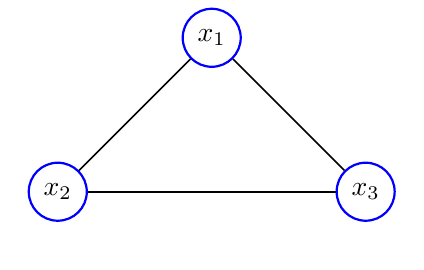
\begin{tikzpicture}
    [node distance = 20mm,
      group/.style={circle,draw=red, thick,}, 
      par/.style={circle,draw=black, fill = black, thick, minimum size = 2pt, inner sep=0pt}, 
      subject/.style={circle, draw=blue, thick},
      fmri/.style={circle, draw=blue, thick, node distance=50mm},
      darc/.style={->, semithick, >=stealth'},
      uarc/.style={-, semithick}]


    \node (x1) at ( 0,0) [subject] {$x_1$};
    \node (x2) [below left=of x1] [subject] {$x_2$};
    \node (x3) [below right=of x1] [subject] {$x_3$};
    \draw[uarc] (x1) to (x2);
    \draw[uarc] (x2) to (x3);
    \draw[uarc] (x1) to (x3);
  \end{tikzpicture}
  \caption{a graph example.}
  \label{fig:graph1}
\end{figure}


  \item New Issues added on Jun 17. We found the clique potential defined by our Dirichlet model is not symmetrical, i.e., $V(x, y) \neq V(y, x)$, and this makes trouble. We take an example graph in figure \ref{fig:graph1}. The Gibbs field is defined as
\begin{equation*}
  P(\vec x) = \frac{1}{Z} \exp \{- [V(x_1, x_2) + V(x_2, x_3) + V(x_1, x_3)]\}
\end{equation*}
The conditional probability of each node are
\begin{align}
  P(x_1 | x_2, x_3) = \frac{1}{Z_1} \exp \{ - [V(x_1, x_2) + V(x_1, x_3)] \}\label{eq:cond1}\\
  P(x_2 | x_1, x_3) = \frac{1}{Z_2} \exp \{ - [V(x_1, x_2) + V(x_2, x_3)] \}\label{eq:cond2}\\
  P(x_3 | x_1, x_2) = \frac{1}{Z_3} \exp \{ - [V(x_1, x_3) + V(x_2, x_3)] \label{eq:cond3}\}
\end{align}
By denifition $x_1$ is Dirichlet given $x_2$ and $x_3$, so $P(x_1|x_2, x_3) = \frac{1}{B(alpha)} \prod_k x_{1k}^{\alpha_k - 1}$, where $\alpha = (x_2 + x_3)/2$. So,
\begin{align}
  P(x_1 | x_2, x_3) &= \frac{1}{B} \exp \{ \sum_k (x_2/2 + x_3/2 - 1)_k \log x_{1k}\}\\
  &= \frac{1}{B} \exp \{ \sum_k x_{2k}/2 \cdot \log x_{1k} + \sum_k x_{3k}/2 \cdot  \log x_{1k} - \sum_k \log x_{1k}\} \label{eq:local}
\end{align}
Comparing \eqref{eq:local} and \eqref{eq:cond1} we have
\begin{equation*}
  V(x_1, x_2) = \sum_k x_{2k}/2 \cdot \log x_{1k}, \quad   V(x_1, x_3) = \sum_k x_{3k}/2 \cdot \log x_{1k}
\end{equation*}
However, above definition of $V(x_1, x_2)$ contradicts with \eqref{eq:cond2}. So, the lack of symmetry makes it difficult to use Dirichlet together with MRF.
\end{itemize}

\section{Current Implenmentation}
Because  of the difficulty of modeling group level as continuous variable, we come back to original proposal of modeling it as a discrete label.

Notation: We use $G$ as the group level label map and $g_s$ is discreate label at site $s \in \mathcal{S}$. $K$ is number of labels, and $\mathcal{K} = \{1, \dots, K\}$ is the set of all lebels.  $Z^j$ is the label map for individual subject $j$, and $\mathcal{J} = \{1, \dots, J \}$ is the set of all subjects. $z_s$ is the label for site $s$. Sometimes I use $z_s^j$ for site $s$ of subject $j$. 

G is MRF, and we use Potts model as
\begin{align*}
  P(G) &= \frac{1}{Z}\exp \{ -U(G)\}\\
  U(G) &= \sum_{(r,s)} \beta [g_r \neq g_s]
\end{align*}

Individual label map $Z^j$ is also a MRF given $G$
\begin{align*}
  P(Z|G) &= \frac{1}{Z}\exp \{ -U(Z|G)\}\\
  P(z_s | g_s, z_{\cN{s}}) &= \frac{1}{Z_s} \exp \{ -U(z_s | g_s,  z_{\cN{s}})\} \\
  U(z_s | g_s,  z_{\cN{s}}) &= \alpha[z_s \neq g_s] + \beta_g \sum_{r\in \cN_s}[z_r \neq z_s]
\end{align*}

At sampling, we need to (1) sample $G$ given $Z$, and (2) sample $Z$ given $G$ and $X$. For sampling $G$ given $Z$ we have
\begin{align*}
  P(g_s|z_s^j, g_{\cN_s}) &\propto P(g_s | g_{\cN_s}) \cdot \beta_g \sum_{r\in\cN_s}[z_r \neq z_s]\\
  U(g_s | z_s^j, g_{\cN_s} ) &= U(g_s) + \sum_j U(z_s^j | g_s) + const\\
  U(g_s | z_s^j, g_{\cN_s} ) &= \beta \sum_{r\in\cN_s} [g_r\neq g_s] + \sum_j \alpha [z_s^j \neq g_s] + const \\
  U(g_s|z_s^j, g_{\cN_s}) &= \beta \sum_{r\in\cN_s} [g_r\neq g_s] + \alpha (J - h(g_s) )
\end{align*}
J is the total number of subjects, and $h()$ is the histogram of label map for all subjects. So we can use above energy function for sampling from $P(G|Z^j)$, and that is equivalent to $P(G|Z^j, X)$.

\section{Von Mises-Fisher Mixture Model Only}
I can also assume a von Mises-Fisher (vMF) mixture modue without MRFs. This is used only for comparison purpose. 

Some scratch notes.
\begin{align*}
  P(z_s = k | x_s, \theta) &= \frac{\pi_k \cV(x_s; \mu, \kappa)}{\sum_k \pi_k \cV(x_s; \mu, \kappa)} = \frac{\pi_k \prod_j \cV(x_s^j; \mu, \kappa)}{\sum_k \pi_k \prod_j \cV(x_s^j; \mu, \kappa)}\\
\log P(z_s = k|x_s, \theta) &=  \log \pi_k + \sum_j \log \cV(x_s^j; \mu_k, \kappa_k) - \log \sum_k \pi_k \left( \prod_j \cV(x_s^j; \mu_k, \kappa_k) \right ) \\
\log P(z_s = k|x_s, \theta) &=  \log \pi_k + \sum_j \log \cV(x_s^j; \mu_k, \kappa_k) - m \\
& - \log \sum_k \left (\pi_k \cdot e^{-m} \cdot  \exp \left \{ \sum_j (\log C^j + \kappa_k \mu_k\T x_s^j)\right \} \right ) \\
&=  \log \pi_k + \sum_j \log \cV(x_s^j; \mu_k, \kappa_k) - m \\
& - \log \sum_k \left (\pi_k \cdot  \exp \left \{ \sum_j (\log C^j + \kappa_k \mu_k\T x_s^j) - m\right \} \right ) \\
m &= \max \{ \sum_j (\log C^j + \kappa_k \mu_k\T x_s^j) \}.
\end{align*}
Introducing $m$ to make sure the exponential function do not overflow. Once I have $\log P(z_s = k|x_s, \theta)$, I can compute $ P(z_s = k|x_s, \theta)$.

\section{Weekly Updates}
\subsection{Nov 21: Test on Scalar Toy Example}
This section is for the experiments of two level scalar data. Group level $G$ is generated by Potts model, and subjects label maps are generated with $G$ as prior. observed scalar voxel intensity is generated from Gaussian distribution. Use MCEM for estimating parameters $\mu$, $\sigma$, $\beta_g$, $\beta_z$. (not yet $\alpha$)

Test (1). \texttt{-v 1 -k 2 -b 20 --inittemp 1 --finaltemp 1 --betag 0 --betaz 0 --alpha 1 --gamma 1} In this case $\beta_g$ reaches to 12 and $\beta_z$ reaches to 6 after 4 EM iteration. The group label map has 0.92 accurary (compared to initial Kmeans on unsmoothed data0.82, and on smoothed data, 0.91). The $\beta$ increases fast, probably the prior distribution take over the posterior $P(Z|G, X)$ and $P(G|Z,X)$, and drives the $G$ and $Z$ smoother at each E step. The estimation of $\beta$ from  smoother label map will be larger and larger, and this make sampling even smoother.

Test (2). \texttt{-v 1 -k 2 -b 20 --inittemp 1 --finaltemp 1 --betag 0 --betaz 0 --alpha 1 --gamma 5 }After increasing the weights of likelihood $P(X|Z)$, $\beta_g$ get stable at around 1.5, and $\beta_z$ stables at 0.9 after 29 iterations. Accuracy is 0.906. Now the likelihood prevents from label map going smoother, and this also prevent $\beta$s going larger by estimation.

In above two tests, the estimation of $\beta$ depends on the relative weights of prior and likelihood term. This is because of the low temperature, such that a slightly difference between the prior and likelihood is magnified by the low temperature, thus make the randomness of the sampling barely happen. While both tests have temperature set to one (amounts to using just the native prior and likelihood), the \emph{low} temperature is relative to the degree of randomness that we want to achieve.

Test (2a). \texttt{-v 1 -k 2 -b 20 --inittemp 1 --finaltemp 1 --betag 0 --betaz 0 --alpha 1 --gamma 3} Similar to test (2) except changing value of gamma. After 30 EM iterations, $\beta_g$ is 1.8 stable, and $\beta_z$ is 0.95 stable. AFter EM finishes, check samples of subjects and group. Subject samples have reasonable randomness, and group samples have less.

Test (3). \texttt{-v 1 -k 2 -b 20 --inittemp 1.8 --finaltemp 1.8 --betag 0 --betaz 0 --alpha 1 --gamma 1} Instead of changing $\gamma$, I can set a higher temperature, so the difference of prior and likelihood is partly canceled by the temperature. The sampling can get reasonable randomness given the difference of prior and likelihood term. AFter 30 EM iterations, $\beta_g$ is 2.64 stable, and $\beta_z$ is .088 stable. Samples for both group and subject level has reasonable randomness. However, the final accuracy is 0.862 for group map, this is less satisfying.

temperature 1.8 is probably the lowest temperature to prevent sampling from going to over-smoothed label map. We do not want temperature too high. Because when it is too high, both prior and likelihood have no influence on the sampling, and the label map samples end up with pure random.

\subsection{Nov 29: MSE of estimates}
Test1: $\alpha = 0.3, \beta_g = \beta_z = 0.5$. $MSE_{\alpha} = 0.0002$, $MSE_{\beta_g} = 0.0006$, $MSE_{\beta_z} = 6.8E-5$.

Test2: Generate data with \texttt{--alpha 0.7 --betag 0.8 --betaz 0.8 -s 200}, and get estimation \texttt{TB: betag = 0.9917, betaz = 0.7963, alpha = 0.6368, Q = 54.796131}. In this scenario, parameter estimation fails to estimate $\beta_g$ and $\alpha$ with reasonable accuracy. Also note the final estimation does not depend on initial value for this Newton's optimization (Changing initial parameter value, still have same final result).

\subsection{Dec 6: Which Parameter To Estimate }
Define the latent variable $Y = (G,Z), Z = (Z^1 \dots Z^M)$ and observation $X$. Define parameter set $\{\alpha, \beta_g, \beta_z, \mu, \sigma\}$. We're looking for $\theta$ that maximize objective function (after Monte-Carlo approximation)
\[
\frac{1}{M}\sum_m \log P(Y^m, X) =  \frac{1}{M}\sum_m \log P(G^m, Z^m, X).
\]
$Y^m$ is one Monte-Carlo sample. The first question is given $Z^m$, $\alpha, \beta_z$ fixed, can we identify $G$ and $\beta_g$ at same time? If there exists a trivial solution of $(G^m, \beta_g)$ that maximize the objective function, the answer will be no (at least when $\alpha$ is small).

The objective function can be written as
\begin{equation}
\frac{1}{M}\sum_m \left( \log P(G^m, Z^m) + \log (X | G^m, Z^m) \right)  = \frac{1}{M}\sum_m \left( \log P(G^m, Z^m) + \log P(X | Z^m) \right) 
\label{eq:GZlogQ}
\end{equation}
I want to fix $Z$ because this is the ideal scenario when the noise of observed data is small such that the sampling of Z always get true subjects labels. If we can prove $(G, \beta_g)$ can not even be identified in this ideal scenario, it can not be identified either when noise is high and $Z$ is not equal to true labels. 

Because $Z$ is fixed, $\log P(X | Z^m)$ is constant to variable $(G, \beta_g)$. The above function is actually 
\[
\frac{1}{M}\sum_m  \log P(G^m, Z^m).
\]
Let $Q = - \log P(G, Z)$. If there is a trivial solution of $(G^*,\beta_g^*)$ to the function $Q$, $(G^1, \dots, G^M, \beta_g)$ will also be a trivial solution to \eqref{eq:GZlogQ} when $G^m = G^*,  \forall m=1\dots M$.

To approximate $P(G,Z)$ by pseudo-likelihood, we assume $(G,Z)$ is a undirected big graph. The conditional probability of a node can be computed in two cases: when the node is on group label map $s\in G$, and when the node is on any subject's label map $s\in Z$. $[cond]$ takes value 1 when the $cond$ is true.
\begin{align*}
  P(G,Z) &= \prod_{s\in G} P(g_s | g_{-s}) \cdot \prod_{s\in Z^j} P(z_s | z_{-s})\\
  &=\prod_{s\in G} \frac{1}{Z_g} \exp \left\{ -\beta_g \sum_{r\in \mathcal{N}_s} [g_r\neq g_s] - \alpha\sum_j [g_s \neq z_s^j] \right\} \cdot \prod_{s\in Z^j} \frac{1}{Z_z} \exp \left\{ -\alpha[g_s \neq z_s^j] - \beta_z\sum_{r\in \mathcal{N}_s} [z_r^j \neq z_s^j] \right\}\\
  Z_g &= \sum_k \exp \left\{ -\beta_g \sum_{r\in \mathcal{N}_s} [g_r\neq k] - \alpha\sum_j [z_s^j \neq k] \right\} \\
  Z_z &=  \sum_k \exp \left\{ -\alpha[g_s \neq k] - \beta_z\sum_{r\in \mathcal{N}_s} [z_r^j \neq k] \right\}
\end{align*}
%% Let $a = \sum_j [g_s \neq z_s^j]$, $b = -\sum_r [g_r \neq g_s]$, $a_1 = -[g_s \neq z_s^j]$, $b_1 = -\sum_r [z_r^j \neq z_s^j]$,
Maximizing $P(G,Z)$ is equivalent to minimize the negative log likelihood (energy function)
\begin{align*}
  - \log P(G,Z) &= \sum_{s\in G} \left ( \beta_g \sum_r [g_r\neq g_s] + \alpha\sum_j [g_s \neq z_s^j] + \log \sum_k \exp \left\{ -\beta_g \sum_r [g_r\neq k] - \alpha\sum_j [z_s^j \neq k] \right\} \right)\\
  &+ \sum_{s\in Z^j} \left(\alpha[g_s \neq z_s^j] + \beta_z\sum_r [z_r^j \neq z_s^j] + \log \sum_k \exp \left\{ -\alpha[g_s \neq k] - \beta_z\sum_r [z_r^j \neq k] \right\}\right)\\
%% &= \sum_{s\in G} \left( -a\alpha - b\beta_g + \log\sum_k e^{a\alpha + b \beta_g}\right) + \sum_{s\in Z^j} \left(-a_1\alpha - b_1\beta_z + \log \sum_k e^{a_1\alpha + b_1\beta_z}\right)\\
%%   &= q_1 + q_2 
\end{align*}

\begin{figure}[htb]
\centering
\includegraphics[width=0.2\textwidth]{figures/simplemrf}
\includegraphics[width=0.4\textwidth]{figures/bothE}\\
\includegraphics[width=0.4\textwidth]{figures/diffE}
\includegraphics[width=0.4\textwidth]{figures/maxE}
\caption{A simple graph and there energy functions. Top left: simple graph with only one subject, and two nodes in each layer. Top right: a plot of $obj_1$ and $obj_2$ over all possible values of $\alpha$ and $\beta_g$. The heights of the meshes are the value of energy function, mapped to color space. We can see when $\alpha = 0$, no matter what values $\beta_g$ takes, $obj_1 < obj_2$, indicating the trivial solution minimize the energy function. Bottom left: the different map $obj_1 - obj_2$. Again we can when $\alpha = 0$, this function is negative over all $\beta_g$. Bottom right: the maximum value over all $\beta_g$ for certain value of $\alpha$. When $\alpha$ is smaller than certain value (here is around 1.5), the trivial solution in case (1) always has smaller energy if we can freely choose $\beta_g$.}
\label{fig:simplemrf}
\end{figure}

Suppose $\alpha$ is very small and even close to zero. In this case the connection between group and subjects label map will be weak and we ignore the $\sum_{s\in Z^j}$ term in above equation. a trivial solution $g_s = const, \forall s \in G$ will have pairwise interaction energy $\sum_r [g_r\neq g_s] = 0, \forall s\in G$. The best $\beta_g$ to minimize $\log \sum_k \exp \left\{ -\beta_g \sum_r [g_r\neq k] - \alpha\sum_j [z_s^j \neq k] \right\}$ will be infinite value. So a $(G=const, \beta_g = \infty)$ is a trivial solution of the above objective function, keeping other variable fixed and $\alpha$ small. That is why the iteration of sampling $G$ and estimating $\beta_g$ will slide into a smoother $G$ and a larger $\beta_g$.

As a example \ref{fig:simplemrf} gives a simple hierarchical graph with only one subject. Both group label map and subject label map have only two nodes $g_r$ and $g_s$. We are going to compare two cases (1) $g_r = g_s = 0, z_r = 1, z_s = 0$ and (2) $g_r = z_r = 1, g_s = z_s = 0$. The only difference between them is the value of $g_r$. That is, when $g_r$'s two neighbors $g_s$ and $z_r$ have different value, will $g_r$ take value of $g_s$ or that of $z_r$.

I want to prove under some conditions of $\alpha$ (i.e. $\alpha$ is smaller than certain value), no matter what values $\beta_g$ takes, the energy function of case (1) is smaller than that of case (2).

The energy function we want to minimize in both cases are
\begin{align*}
obj_1 &= 2\alpha + 2\beta_g + \log (1 + e^{-\alpha - \beta_g}) + \log (e^{-\alpha} + e^{-\beta_g}) + \log (e^{-\alpha} + e^{-\beta_z} ) + \log (1 + e^{-\alpha - \beta_z})\\
obj_2 &= 2\beta_g + 2\beta_z + 2 \log (e^{-\beta_g} + e^{-\alpha}) + 2 \log (e^{-\alpha} + e^{-\beta_z})
\end{align*}
There is no apparent analytical solution of $obj_1 - obj_2 = 0$ in order to find the relationship of $\alpha$ and $\beta_g$, so we have to draw the value of $obj_1$ and $obj_2$ over all possible $\alpha$ and $\beta_g$ in a domain. The bottom right plot of \ref{fig:simplemrf} shows when $\alpha$ is smaller than certain value, the trivial solution in case (1) always has smaller energy than the other solution.

If $\alpha$ is also an variable to be estimated, from the bottom right of figure \ref{fig:simplemrf}, we see a large $\alpha$ together with the normal solution in case 2 have less energy than a small $\alpha$ and trivial solution. In this particularly simple example, the estimation of alpha would be larger than 1.5, which means the group and subject labels are more than 95\% same. In real world scenario, it is unknown whether this estimation is what we expect.

\textbf{Estimation of $\alpha$:} We can keep $\beta_g = \beta_z$ to a fixed value and estimate $\alpha$ and $G$ at same time. Can this estimation have a trivial solution where $\alpha = 0$ and $G$ have all constant labels?

Some preliminary test on real data (16 R subjects) indicates that  $\alpha$ estimation is not good. Once the $\alpha$ estimation diverges, the $G$ map is also affected by the bad $\alpha$ parameter. We need regularize  $\alpha$ by introducing prior distribution (with hyper parameters) on $\alpha$.


\begin{figure}[htb]
\centering
\includegraphics[width=0.4\textwidth]{figures/testalpha_beta_1}
\caption{The energy function of two cases of G,  over all value of $\alpha$. }
\end{figure}

\subsection{Jan 9 -- Jan 13: Same Subject Label Map}
\textbf{Scenario 1} First, when generating synthetic label map $(G, Z)$, use a large enough $\alpha$ such that all subjects and group label map are same. When $\alpha = \beta_g = \beta_z = 2.0$. The mean time series are generated with a AR process with coefficient $\varphi = 0.8$ and noise variance $\sigma_{\epsilon}^2 = 1$. The variance of each voxel in the mean time series is $\sigma_{\epsilon}^2 / (1- \varphi^2) = 2.9$. To generate observed time series, I add Gaussian noise ($\sigma = 5$) to each time point of each time series. The signal-to-noise ratio (SNR) is $3/5 = 0.6$. 

Besides the SNR, the correlation between the mean time series also have big impact on the separability of different clusters. For this synthetic data,  the mean time series are supposed to be un-correlated, and the actual correlations between any pair of mean time series range from -0.17 to +0.38 (the seond largest correlation is 0.23).  Such correlation is small than those computed from real fMRI time series (not 100\% sure). So, despite of a low SNR, this synthetic data is still separable.

In the synthetic data, the subjects and group map are 98\% same. K-means clustering gives a group label map that is 100\% consistent with the ground truth.

My \texttt{groupmrf} program take the K-means clustering as initial group and subject label map. Initialize $\beta_g$, $\beta_z$ and $\alpha$ with true value used for generating the data. burning period set to 20, number of MC samples is 5.  Since we do not test the randomness of sampling in this scenario, it is not important that all MC samples are the same, and the number of MC samples have no effect on final results. The $\gamma$ parameter set to 0.1, meaning $\log P(X|Z)$ is downweighted to one tenth of the original value.

After 30 EM iteration, we have $\alpha = 1.84, \beta_g = \beta_z = 2.36$. The final group label map is 100\% consistent with the truth. The estimated subject 1's label map is 99.9\% consistent with the truth. It is not 100\% correct, and the incorrect labeling happens on the boundary between two clusters. This is probably because of the downweighting of $\log P(X|Z)$, and the spatial smoothness prior outweights the $\log P(X|Z)$, so the labeling prefer spatial smooth map ranther than trying to be consistent with the data.  All three parameters do not change significantly after 2 EM iteration. So 30 EM iterations is really not necessary in this particular scenario.


\textbf{Scenario 2: } In this scenario we keep everything else same with scenario 1, but decrease $\alpha$ when generating synthetic data. Choose $\alpha = 0.3, \beta_g = \beta_z = 2.0$, and scan both $G$ and $Z$ map 1000 times to obtain the synthetic label map. In the generated synthetic data, group and subjects label map have consistency ranging from 71\% to 96\%, and most are between 90\% and 95\%. If we estimate parameters from this single sample, The estimated parameter values are $\alpha = 0.24, \beta_g = \beta_z = 2.02$. 

\texttt{K-means} gives a clustering that is 87.4\% correct for group label map. \texttt{groupmrf} gives a group label map with 87.5\% correct rate. For subject label map estimation, \texttt{groupmrf} gives estimation with accuracy as 86.5, 82.0, 77.7, 85. 6, etc. The estimated parameters are $\alpha = 0.89, \beta_g = \beta_z = 2.01 $. The $\beta$ parameter match the true value pretty well, but the $\alpha$ does not, probably because of the inaccurate subject label map.

\textbf{Scenario 2a: }  The synthetic data are same with scenario 2, and the K-means clustering are also same. Since in scenario 1, the estimated subject label maps have low accuracy, we will add weights of $\log P(X|G,Z)$ in this scnario and set $\gamma = 1$ (so the posterior will be the standard Bayesian posterior). I will expect the subject label map have a good match to the truth since the $\log P(X|G,Z)$  is so strong in its default $\gamma$ value. 

\texttt{groupmrf} estimation of the parameters are $\beta_g = \beta_z = 1.92, \alpha = 0.53$. The group label map is 86\% same with the truth, and subject label map accuracy are 81.9, 76.9, 85.5, 85.3, 80.8, etc. This result is a little beyond my expectation. I would expect a higher accurary on subject label map. The possible reason is the SNR is not big enough, and the likelihood is still not strong enough for the individual subject label map to get correct.


\textbf{Scenario 2b: } Based on the previous scenario 2a, I increase the SNR by setting the additive noise $\sigma = 1$. So the SNR is $3/1 = 3$. Everything else kept same to scenario 2a, the K-means gives 98\% accuracy, which means the time series data is good enough to get subject label map correct.

\texttt{groupmrf} estimates of the parameters are $\alpha = 0.31, \beta = 2.03$, a pretty good estimation. The $G$ map has 100\% accuracy compared to truth, the individual subject label map accuracy are 91.1\%, 86.3\%, 93.9\%, 95.1\%, 70.8\%, 69.8\%, 92.8\%, 93.4\%, 92.2\%. 

The parameter estimation is good in this scenario, but the estimation of individual label map is not. Theoretically, if the log likelihood $\log p(X|G,Z)$ is strong enough, the clustering will be just like standard mixture of Von-Mises Fisher, and the clustering for each subject should have high accuracy. Need double check this issue.

\subsection{Jan 16 -- Jan 20}
I made a few fixes: 
\begin{itemize}

\item the subject file naming conventions issue. Now the program supports number of subjects larger than 10, and the output files match input files. 

\item Make sure the log likelihood (after pseudo likelihood and MC approximation) does increase after each sampling step and parameter estimation step. Since sampling step is performed at very low temperature, it is just the up-hill climbing on the log likelihood function. That means, at each voxel, the label with largest posterior probability will be chosen with 100\% probability, i.e. no randomness in sampling. This guarantee the loglihood always increase with each sampling. I will test randomness of the sampling in next week. For parameter estimation, I tested the estimation of both prior parameters $\alpha$, $\beta$, as well as von Mises parameters $\mu$ and $\kappa$ increase likelihood function. 

\item Use a new routine \texttt{subkmeans} to estimation the label map for each subjects separately, and use another new routine \texttt{alignlabels} to rearrange/permute the subject maps' labels such that it is consistent with estimated group label map computed by \texttt{initmrf} (K-means). Here \emph{consistent} means same region between two label maps have same labels, and if it they do not, I permute the labels to align them.

\end{itemize}

After fixing the critical error in \texttt{projectfmri} ( I still need to look into the bug if I have time), here is a scenario of more interest.

\textbf{Scenario 3: } Generate $(G,Z)$ label map with $\alpha=0.3$, $\beta=2$ and scan 500 times. The rand index value between 16 subject map and group map are most between 78 to 84. Generate observed fmri time series by adding Gaussian noise with variance 100. \texttt{subkmeans} estimate  subject label label maps with accuracy around 88\%, and \texttt{initmrf} use kmeans on all subject to estimate a group label map with 95\% accuracy. 

Our \texttt{groupmrf}'s group label map has 96\% accuracy, slight improved than the K-means. By looking at the image, \texttt{groupmrf}'s group label map has a clear boundary and looks better than K-means's. The subject label maps are significantly better than \texttt{subkmeans}.

Todo list: Probably next step is to test the spatial smoothing. I want to compare K-means on spatial smoothed data with \texttt{groupmrf} on the data without smoothing. I want to assume the spatial dependency of the additive Gaussian noise on fmri, so I want to generate noise, spatial smooth the noise and then add the noise on the mean time series. I expect to see spatial smoothing on observed fmri image does not help much since the noise are already dependent on their spatial neighbors. I expect to see our mrf works better. 

I also want to run ICA on the data in scenario 3. And I need to replace Metropolis sampling with Gibbs sampling (though is seems not a high priority task).

\subsection{Jan 23 -- Jan 27}
ADHD200 data sets have multiple subsets from various sites. Take University of Pittsburgh subsets for example, it has around 90 subjects. all of them are normal controls, but some of them do not have good quality on fmri data according to the description of the data set. 66 subjects have good quality on resting state scans, and I plan to use this sub dataset of 66 subjects for our study. I used the preprocessing scripts provided along with the dataset. That includes motion correction, registration to template space, slice timing correction, band-pass filter, removing the nuiance parameters (white matter, CSF, motion parameters) by regression, and spatial smoothing. I can extract both spatial smoothed and un-smoothed fmri data from the output of the script.

From each subject's tissue segmentation map, I compute the average gray matter segmentation map over all subjects, and threshold that to get a binary mask of gray matter. This is used in the following clustering.

Then I run \texttt{subkmeans} on each subjects spatially smoothed data to get the initial label map. I used smoothed fmri data because I can get a better initial label map than using un-smoothed fmri data. The maps look OK. Next step is to run \texttt{initmrf} get a group label map by K-means. The routine is still running and will be done by Friday night.

\textbf{Test on R dataset: } After fixing the bugs in \texttt{projectfmri}, I re-run the K-means to get a new group label map. I can see the difference between this new estimated map with the label map before fixing the bug, but it is difficult to tell which is better. 

After I permute the labels of estimated subject labels computed from \texttt{subkmeans} to be consistent with the estimated group label map, the percentage of consistent labels are roughly 50\%, but the rand index is significantly higher, around 70\%. Though I know there is no correspondence between these two indices, this is still strange enoug and worth looking into.

The first run of \texttt{groupmrf}, I set $\alpha = 0.4, beta = 2, \gamma=1$. Unsmoothed fmri data is used. Result: subject label maps are divided into small regions, probably because of the unsmoothed fmri. It is also probably because the data likelihood is stronger than prior, such that MRF does not have chance to have effect on final label map.

The second run, I changed $\gamma=0.1$. I can see the subject label maps are in big chunks, but ...

-- Rewrite parameter estimation code so it runs in parallel for all subjects.

\subsection{Jan 30 -- Feb 3}
\textbf{Test1:} Last week we conclude we might still have to use smoothed data, so in test1 I use smoothed data in \texttt{groupmrf}. I also fix group label map by not sampling any voxles in it. This is same to empirical Bayesian method in spirit. In empirical Bayesian, the parameter in prior distribution is estimated by maximizing the likelihood of the marginal distribution of the data. Our group label map can be seen as a hyper-parameter estimated from the data, and are kept fixed thereafter. By chaging $\gamma$ -- the wieghts of data likelihood term, I found a $\gamma$ betwen 0.2 and 0.3 can give subject label maps with noticeable difference to group map but still meaningful.

\textbf{Test 2:}

\textbf{Test 3:} I tried to apply Gift ICA toolbox on our \emph{synthetic} data set but failed. The Gift report eigen-decomposition error and exit, without generating any results. This is probably because the model we used to generate the synthetic data violate Gift assumption of the real fMRI data. Also tried fsl's melodic routine and also failed for unknow reason.

\textbf{Test 4: } Downloaded canICA package and install it, run it on our R data set. Get stability maps but hard to explain. The package are written in Python and may be difficult to hack into in order to print more information.

\textbf{Test 5: } Is trying \texttt{freesurfer} for visualization purpose. However, it seems \texttt{freesurfer} need a whole data processing pipeline to be done in their software. It might be difficult to just plug in our segmentation map into it for simple visualization.

Some thoughts: Make comparison to ICA approach is difficult, since the clustering approach and ICA approach are two very different concept. Our clustering is a hard labeling method, but ICA generate a component map, which is the mixing weights of the indepedent components. A normalization and thresholding on the map is what people usually do.

It would be easier to compare our method with other clustering-based methods.

meeting minutes: estimation label map; Stability test; Compare to other methods.

\subsection{Feb 6 - Feb 10}
\texttt{init\_7} is before I fixed the bug in \texttt{projectfmri}, and \texttt{init\_7a} is after the bug fix. Since the DMN looks not as good as before the bugfix. I revert the source file of \texttt{projectfmri} and try to reproduce \texttt{init\_7}. I save the file as \texttt{init\_7b}. It ends up that \texttt{init\_7b} still looks not good on DMN. That means I can not reproduce \texttt{init\_7}. Another reason is the seed value of the \texttt{initmrf} routine.

Also using old version of projectfmri routine and run initmrf with 6 clusters. Save this as init\_6b.

Then I found in conn configuration there is a mistake: I incorrectly set PCC and MPFC as a confound and remove their effects from all over the brain voxels. After correcting it, run the initmrf again and save the file as init\_7c. Wait to see the result...ok the results looks good, almost same as init\_7. So this issue is solved.

Also checked the subkmeans applied on concatenated time series, and found it is almost same as the initmrf output. In the future subkmeans can be used as the group K-means routine to replace initmrf.

For ADHD data, I want to see if 20 iterations of K-means for initmrf routine really works better, so I run initmrf again with only 2 K-means iterations and save the file as init\_7a. Conclusion: 2 iterations get similar result with 20 iterations. Therefore it is not necessary to run 20 iterations.

Also estimate $\beta$ on ADHD data and found $\beta$ stable at 1.7. If I initialize $\beta$ to 2.0, it will reach 1.7 at the first 3 EM iterations. This is probably because the spatial smoothness of the data. The results looks fine.

Next step, estimate $\alpha$ and $\beta$ parameter both. Result: $\alpha$ estimation is close to zero, and sometimes go below zero. This is because each subject's data likelihood term is so strong that it pull the subject labels away from group label map. $\gamma = 0.3$ in this case. I could not find a good $\gamma$ value such that subjects labels are differnt from group label map but not too different such taht $\alpha$ gets good estimation.

Also begin the paper draft: \url{https://gforge.sci.utah.edu/svn/confield/papers/miccai2012}

Wrote a python routine to draw bootstrap samples from the 66 subject ADHD dataset. I did a preliminary test: each bootstrap sample is a subset of the original dataset. I choose 5 subjects in each bootstrap sample, and choose 10 such subsets to run the K-means and groupmrf routine. Results: looks not bad, but need further tests. Issues: 1) how many subjects in one subsets? 2) How to get consensus from the bootstrap clusterings.

For issue 2) we can use Parasaran's consensus method. We don not want to elaborate his method (and we do not have page space to do that). We can just plug in his method and the paper looks better. parasan can be one of the authors.

\subsection{Feb 13 -- Feb 20}
Meeting minutes: Tune $\gamma$. Compute mean of posterior label map. 

The test1 still have too much difference on subjects level. I either need to decrease $\gamma$ or increase $\alpha$ so subject label maps have less change.

Synthetic data: try to beat K-means on smoothed data. Very difficult. Generate data with $\alpha=0.5$ but seems not work well. Re-generate with $\alpha=0.7$.

Implemented Normalized cuts. First apply N-cuts on each subjects, convert the label map to a clustering matrix of N by N. Sum the matrix over all subjects, thresholding, and do second N-cuts clustering. The results looks not reasonable, I couldn't even find the DMN on the group network. I want N-cuts to give reasonble results to compare with. Will try again with different parameter. Also the region of clustering (gray matter mask) seems have big impact on the results (weird). I'll also play with different masks. 

ADHD data: parameter estimation of $\alpha$ with strong prior. Underway.

\subsection{Feb 20 - Feb 27}
We conclude the mask file for ADHD have too many gray matter voxels. New way to get the mask 1) bet the nihpd 1mm t1w file. 2) fast the t1w file to get the gray matter segmentation image. Looks good. 3) fslmaths to subsample the gray matter tissue. The mask looks not good. Small holes. If I blur the image with Gaussian filter, I can fill the small holes, but in that case the image will be no difference from my current average gray matter from individual subjects. OK probably I should just use the original mask, but thresholded with higher value.

    

\bibliographystyle{plainnat}
\bibliography{ref}
\end{document}  
